

% 2015/11/7


% new features:
% custom distances
% data(galbraith), .....




\documentclass[11pt,a4paper]{article}
\usepackage[utf8]{inputenc}
\usepackage[english]{babel}
\usepackage{microtype}
\usepackage{graphicx}
\usepackage{color}
\usepackage{hyperref}
\usepackage{alltt}
\usepackage{geometry}
    \geometry{left=25mm,right=40mm,top=22mm}


\hypersetup{
  pdftitle={stylo: a package for stylometric analyses},
  pdfauthor={Maciej Eder, Jan Rybicki, Mike Kestemont},
  pdfsubject={R package 'stylo'},
  pdfkeywords={computational stylistics,} {stylometry,} {authorship attribution},
  colorlinks=true,        % false: boxed links; true: colored links
  linkcolor=black,        % color of internal links
  linktoc=all,            % both sections and subsections linked
  citecolor=black,        % color of links to bibliography
  filecolor=black,        % color of file links
  urlcolor=black          % color of external links
}



\frenchspacing


\definecolor{darkred}{rgb}{0.8,0,0}  
\definecolor{darkgreen}{rgb}{0,0.8,0}
\definecolor{darkblue}{rgb}{0,0,0.8}

\definecolor{mygreen}{rgb}{.36,.37,.08} % rgb: 93 95 22
\definecolor{myblue}{rgb}{.07,.28,.4} % rgb: 18 73 102
\definecolor{myyellow}{rgb}{.75,.54,.12} % rgb: 193 138 31
\definecolor{myred}{rgb}{.52,.03,.3} % rgb: 133 9 79
\definecolor{myorange}{rgb}{.6,.26,.05} % rgb: 155 66 12


\def\underscore{\raisebox{-.8ex}{-}}
\def\margin#1{\marginpar{\textcolor{blue}{\footnotesize\tt #1}}}

%\usepackage{marginnote}
%\def\margin#1{\marginnote{\textcolor{blue}{\footnotesize\tt #1}}}

\def\code#1{{\tt #1}}

\def\textquotedbl{"}



\title{{\tt `Stylo'}: a package for stylometric analyses}

\author{Maciej Eder\\ {\footnotesize Pedagogical Univ. of Kraków}
    \and Jan Rybicki\\ {\footnotesize Jagiellonian University}
    \and Mike Kestemont\\ {\footnotesize University of Antwerp}
    }





\begin{document}


\maketitle

\begin{center}
  
\includegraphics[width=0.2\linewidth]{img/csg.png}
\end{center}

\vglue\baselineskip

\hrule
\begin{abstract}
The \code{`stylo'} package (Eder et al. 2013) provides
easy-to-use implementations of various established analyses in the
field of computational stylistics, including non-traditional authorship
attribution, genre recognition, style development (``stylochronometry''),
etc. The package includes a number of explanatory methods provided
by the function \code{stylo()} (multidimensional scaling, principal
component analysis, cluster analysis, bootstrap consensus trees).
Addtionally, a number of supervised machine-learning methods are available
via the function \code{classify()} (Delta, support vector machines,
naive Bayes, \textit{k}-nearest neighbors, nearest shrunken centroids). The
\code{rolling.delta()} function analyses collaborative works and
tries to determine the authorship of fragments extracted from them. 
The function \code{rolling.classify()} offers a more flexible interface
to sequential classification of collaborative works.
The \code{oppose()} function performs a contrastive analysis between
two given sets of texts: among other things, it generates lists of words 
significantly \emph{preferred} and \emph{avoided} by one or more authors 
in comparison to the texts by another author (or a set of them). 
\end{abstract}


% a tiny trick to typeset keywords as if they were an abstract
\global\long\def\abstractname{Keywords}

\begin{abstract}
\noindent stylometry, computational stylistics, authorship attribution,
cluster analysis, dendrogram, bootstrap consensus trees, PCA, MDS,
\textit{k}-NN, SVM, NSC, naive Bayes, Delta, Zeta, rolling stylometry
\end{abstract}

\bigskip

\hrule

\bigskip

\tableofcontents

\bigskip\bigskip



\section{Introduction}

Stylometric studies, in all their variety of material and method,
have two features in common: the electronic texts they study have
to be coaxed to yield numbers, and the numbers themselves have to
be processed via statistics. Sometimes, the two actions are two independent
parts of a given study. To give the simplest example, one piece of
software is used solely to compile word frequency lists; then, one
of the many commercial statistics packages takes over to extract meaning
from this mass of words, draw graphs etc.

Yet, as stylometrists have begun to produce statistical methods of
their own – to name but a few, Burrows’s Delta, Zeta and Iota (Burrows,
2002, 2007) and their modifications by other scholars (Argamon, 2008,
Craig and Kinney, 2009, Hoover, 2004a, 2004b) – commercial software,
despite its wide array of accessible methods, becomes something of
a straightjacket. This is why a number of dedicated stylometric solutions
have appeared, targeting the specific analyses frequently used in
this community. Hoover’s Delta, Zeta and Iota Excel spreadsheets are
pioneering examples of this approach (Hoover, 2004b). Constantly developed
since 2004, they have at least two major assets: they do exactly what
the stylometrist wants (with several optional procedures) and they
only require fairly standard -- although proprietary -- spreadsheet
software. This has been especially helpful for uses in specialist
workshops and classrooms: the student only needs additional (and,
often, free) software to produce word frequency lists and (s)he is
ready to go. Yet Excel imposes one important limitation: it is very
demanding from the point of view of memory usage. Moreover, the two-stage
nature of the process (a separate piece of software prepares word
lists that can be later automatically imported into the spreadsheet)
might be problematic, because it takes an experienced Visual Basic
programmer to make Excel itself extract the various frequency dictionaries
needed.

In this respect, Juola's JGAAP can directly import texts in a variety
of formats and perform a variety of authorship attribution tasks using
an impressive variety of statistical methods (Juola et al., 2008).
These can be further expanded by experienced programmers in Java.
Java is also the language of another software solution which takes
an even broader approach: Craig's Intelligent Archive is able to perform
a number of standard stylometric procedures, but it can also be used
as a corpus organizer. Once the initial work of registering texts
is done, it enables a versatile combination of individual texts and
groups of texts (Craig and Kinney, 2009).

Since contemporary stylometry uses either stand-alone dedicated programs
custom-made by stylometrists, or applies existing software, the \code{stylo}
package can be situated somewhere in-between: the powerful open-source
statistical programming environment R provides, on the one hand, the
opportunity of building statistical applications from scratch, and,
on the other, allows less advanced researchers to use ready-made scripts
and libraries (cf. http://www.R-project.org). 
In our own stylometric adventure with R, one of the
aims was to build a tool (or a set of tools) that would combine sophisticated
state-of-the-art algorithms for classification and/or clustering with
a user-friendly, ``point-and-click'' interface. In particular, we wanted
to implement a number of popular multidimensional methods to be used
by scholars without advanced programming skills. It soon became evident
that once our R scripts were provided with a graphical user interface
and modest documentation, they lent themselves well to classroom use.
In our experience, this suite of tools offers an excellent way to
work around R's typically steep learning curve, without losing anything
of the power of the environment -- namely R's considerable computing
power and speed.

A crucial point in building the interface was to make sure that all
stages of a typical stylometric analysis -- from loading texts to
visualizing the results -- could be performed from within a single
function. The \code{stylo()} function, for instance, does all the
work: it processes electronic texts to create a list of all the words
used in all texts studied, with their frequencies in the individual
texts; normalizes the frequencies with \textit{z}-scores (if applicable);
selects words from the desired frequency ranges; performs additional
procedures that might improve attribution, such as Hoover's (2004a,
2004b) automatic deletion of personal pronouns and ``culling'' (automatic
removal of words too characteristic for individual texts); compares
the results for individual texts; performs a variety of multivariate
analyses; presents the similarities/distances obtained in tree diagrams;
and finally, produces a bootstrap consensus tree (a new graph that
combines many tree diagrams for a variety of parameter values). It
was our aim to develop a general platform for multi-iteration stylometric
tests; for instance, an alternative script derived from the function
\code{classify()} produced heatmaps to show the degree of Delta's
success in attribution at various intervals of the word frequency
ranking list (Rybicki and Eder, 2011).

The last stage of the interface design was, firstly, to add a GUI
(since some humanists might be allergic to the command-line mode provided
by R) and, secondly, a host of various small improvements (like saving
and loading the parameters for the most recent analysis, a wide choice
of graphic output formats, etc.). Nevertheless, advanced users could
still easily switch off the GUI and embed the functions provided by
the ``stylo'' library in their own scripts.


\section{Installation}

Make sure you are connected to the internet. Launch R. Type \code{install.packages("stylo")}
in the console. Whenever you start a new R session, type \code{library(stylo)}.
This will automatically load all the functionality provided in the
package (see below). If you are very lazy and only use R for stylometric
purposes, you can find your \code{Rprofile.site} configuration file 
(in \code{R/R-<your R version here>/etc}), open it with administrator privileges
and insert the line \code{library(stylo)} there. In this case, the
``stylo'' library will be loaded at the start of each R session and you
can start invoking the particular functions right away.


\section{Functions provided}

The most important tools included in this package are distributed
over the following functions:

\begin{itemize}
  \item \code{stylo()}
  \item \code{classify()} 
  \item \code{oppose()} 
  \item \code{rolling.delta()}
  \item \code{rolling.classify()}
\end{itemize}

The next sections of this manual describe these four functions together
will all the different input options they can take. If you want to
get a general overview of these four functions, type \code{help(stylo)},
\code{help(classify)}, etc., and a help window will appear. More
advanced users might be interested in some other functions
provided by the library. Generally speaking, they are a great deal
of lower-level functions which are called automatically from inside
the upper-tier functions, such as \code{classify()}, \code{oppose()},
etc. This lower-level functionality can of course be used for developing
your own scripts and functions. These include:

\begin{itemize}
  \item \code{assign.plot.colors} 
  \item \code{define.plot.area} 
  \item \code{delete.markup}
  \item \code{delete.stop.words}
  \item \code{dist.argamon}
  \item \code{dist.cosine}
  \item \code{dist.delta}
  \item \code{dist.eder}
  \item \code{dist.simple}
  \item \code{draw.polygons}
  \item \code{gui.classify} 
  \item \code{gui.oppose}
  \item \code{gui.stylo} 
  \item \code{load.corpus.and.parse} 
  \item \code{load.corpus} 
  \item \code{make.frequency.list}
  \item \code{make.ngrams} 
  \item \code{make.samples} 
  \item \code{make.table.of.frequencies} 
  \item \code{parse.corpus}
  \item \code{parse.pos.tags}
  \item \code{perform.culling}  
  \item \code{perform.delta}
  \item \code{perform.knn}
  \item \code{perform.naivebayes}
  \item \code{perform.nsc}
  \item \code{perform.svm}
%  \item \code{print.stylo.corpus}
%  \item \code{print.stylo.data}
%  \item \code{print.stylo.results}
  \item \code{stylo.default.settings} 
  \item \code{stylo.pronouns} 
%  \item \code{summary.stylo.corpus}
%  \item \code{summary.stylo.results}
  \item \code{txt.to.features} 
  \item \code{txt.to.words.ext} 
  \item \code{txt.to.words} 
  \item \code{zeta.chisquare}
  \item \code{zeta.craig}
  \item \code{zeta.eder}
\end{itemize}

In most cases, these lower-level functions provide very basic processing
functionality and they are therefore not intended to be invoked by
everyday users. Hence, they will not be discussed in this manual.
However, if you are interested how they work and how to use them,
you can invoke the help pages for these functions: \code{help(load.corpus)},
\code{help(make.ngrams)}, etc. Help pages routinely contain some
insightful examples as to how to use the code: refer to them if you
want to understand what a particular function does. The examples can
be copy-pasted into an active R console. (Don't be afraid of the lines
`\code{\#\#~Not run}' -- they prevent R to run some automatic
checks on interactive functions; you can use these examples safely).

Apart from functions, the package \code{`stylo'} (ver. >0.6.1) contains 
three datasets that can be used to start playing with stylometric methods 
without any actual texts. The datasets are as follows:

\begin{itemize}
  \item \code{novels}
  \item \code{galbraith}
  \item \code{lee}
\end{itemize}

The first dataset contains 9 full-size novels by Jane Austen and 
the Bront\"e sisters. The second and the third set contains computed
tables of word frequencies for 26 and 28, resp., contemporary novels 
that for copyright-related reasons could not be made available in 
their original format. A detailed description of the datasets 
can be retrieved via \code{help(novels)}, \code{help(galbraith)}
and \code{help(lee)}. 

\section{stylo()}

This is currently the main tool in the package. The function \code{stylo()}
is meant to enable users to automatically load and process a corpus
of electronic text files from a specified folder, and to perform a
variety of stylometric analyses from multivariate statistics to assess
and visualize stylistic similarities between input texts. This function
provides explanatory analyses; any users interested in machine-learning
supervised methods might want to skip this section and go to 
\code{classify()}, below.

\code{stylo()} will typically be used to produce a most-frequent-word
(MFW) list for the entire corpus. Next, it will acquire the frequencies
of the MFWs in the individual texts to create an initial matrix of
words (rows) by individual texts (columns): each cell will contain
a single word's frequency in a single text. Subsequently, it will
normalize the frequencies: it selects words from the the desired frequency
ranges for an analysis (this is also saved to disk as 
\code{table\underscore{}with\underscore{}frequencies.txt}
and it will perform additional processing procedures (automatic deletion
of personal pronouns and culling, see 4.3.5 below) to produce a final
wordlist for the actual analysis (this information is saved to disk
in the current working directory as \code{wordlist.txt}. It then
compares the results for individual texts, performing e.g. distance
calculations and using various statistical procedures (cluster analysis,
multidimensional scaling, or principal components analysis). Finally,
the function will produce graphical representations of distances between
texts and it will write the resulting authorship (or similarity) candidates
to a logfile (\code{results.txt}) in the current working directory.
When the \code{consensus tree} option is selected, the script produces
virtual cluster analyses for a variety of parameters, which then produce
a final diagram that reflects a compromise between the underlying
cluster analyses.


\subsection{Corpus preparation}

\begin{figure}
  \centering
  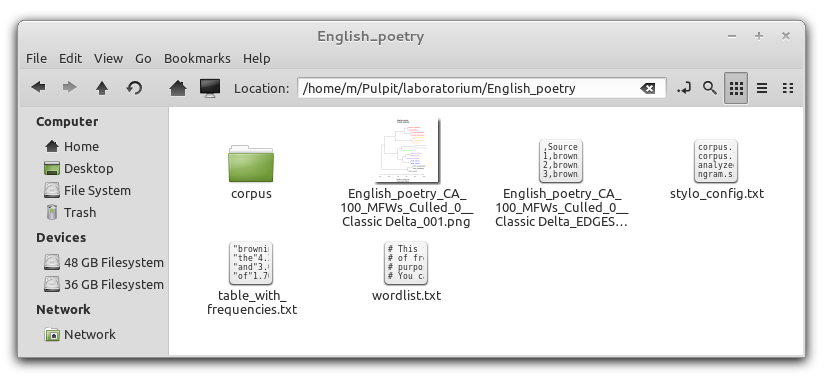
\includegraphics[width=0.85\linewidth]{img/stylo_corpus1.png}
  \caption{Working directory containing a subdirectory \code{corpus} and some files generated by the function \code{stylo()}.}
\end{figure}

The procedure of loading corpora as described immediately below is probably the best way to start doing your first analyses. However, experienced users of R sooner or later will discover that input data structures (corpora, vectors of features, tables of frequencies) can be passed as R objects directly from, say, other functions, without any interaction with texts files. Refer to section 9.1 for details.

Each project requires a separate and dedicated working folder. You
will want to give it a meaningful name (like \code{SanskritPoetry11}
rather than \code{Blah-blah}), since the name of the folder will
appear as the title in your graphs generated by the function. By default,
the results of your analyses and other useful files will be written
automatically to this folder. The actual text files for your analyses
must be placed in a subfolder in the working directory, named \code{corpus}
(Note: all file names are case sensitive!). All functions in this
tool suite expect to find at least two input texts for their analyses.

The text files need to follow the following naming syntax: \code{category\underscore{}title.txt}.
For people working in authorship attribution, the \code{category}
will capture a text's authorial signature; other users, perhaps interested
to compare a translators' styles, should name their files \code{translatorname\underscore{}title.txt}.
Likewise, if you are looking for stylistic similarities between writers
of the same gender, use \code{gender\underscore{}title.txt},
etc. It is really important to use an underscore ``{}\code{\underscore}''
(underscore) as a delimiter: e.g. colors on the final graphs will
also be assigned according to strings of characters up to the first
underscore in the input files' names. (For further details and examples,
type \code{help(assign.plot.colors)}). Consider the following examples,
in which the classes are the authors' names and authors' gender, respectively:

\medskip

\code{
\noindent
\textcolor{darkgreen}{ABronte}\underscore Agnes.xml \\
\textcolor{darkgreen}{ABronte}\underscore Tenant.xml \\
\textcolor{darkred}{Austen}\underscore Emma.xml \\
\textcolor{darkred}{Austen}\underscore Pride.xml \\
\textcolor{darkred}{Austen}\underscore Northanger.xml \\
\textcolor{myyellow}{Conrad}\underscore Nostromo.xml \\
\textcolor{myyellow}{Conrad}\underscore Lord.xml \\
\textcolor{darkblue}{Dickens}\underscore Pickwick.xml \\
\dots
}

\medskip

\code{
\noindent
\textcolor{darkred}{M}\underscore Conrad\underscore Lord\underscore Jim.txt \\
\textcolor{darkred}{M}\underscore Joyce\underscore Dubliners.txt \\
\textcolor{darkgreen}{F}\underscore Woolf\underscore Night\underscore and\underscore day.txt \\
\textcolor{darkgreen}{F}\underscore Woolf\underscore Waves.txt \\
\dots
}

\medskip


Everything that comes after the underscore (say, the short titles
of novels) can be followed by any other information. Be careful with
long names, however, since these might not fit in the graphs that
will be generated. The texts must either be \textit{all} in plain
text format, or \textit{all} in HTML, or \textit{all} in TEI-XML (the
latter two options have not been extensively tested so far, and should
be used carefully). 

A concise remark about possible encoding issues should also be added. 
If the operating system you use is Linux or Mac, you just need to make 
sure the texts are all in UTF-8 (aka Unicode). If your operating system 
is Windows, you have two options. Firstly, you might want to save all 
the texts in ANSI codepage, but you have to tread carefully if your 
machine runs one charset, say, Central European (1250) and your texts 
are in the Western European codepage (1252); in this respect, for 
instance, French is notoriously difficult (\emph{nous sommes vraiement 
désolés}). Alternatively, you can convert your texts into Unicode 
(a variety of freeware converters are available on the internet), 
and to use an appropriate encoding option when launching the function, 
say, \code{stylo()} either by clicking the ``UTF-8'' button on GUI 
(beginners), or passing the argument \code{encoding = "UTF-8"} directly 
to the function (advanced users).



\subsection{Starting the function}

Start up R. At the prompt (where you see the cursor blinking), move
to your folder (the main folder you will be working in, \textit{not}
the \code{corpus} subfolder) using the command \code{setwd()}.
E.g.:

\medskip{}
\code{setwd("/Users/virgil/Documents/disputed-works-of-mine")}
\medskip{}


\noindent You can use either absolute paths (as in the above example),
or relative ones, i.e. you can navigate directly from the current
working directory. If you want to go, say, two levels up and then
descend to a folder \code{first\underscore experiment},
type:

\medskip{}
\code{setwd("../../first\underscore experiment")}
\medskip{}


You can always check you current working directory typing \code{getwd()}.
(If you use R app for Windows, you can set your directory by clicking
the \emph{File} menu: see Fig.~1; Mac OS users -- click the \emph{Misc}
menu on your R console). Call the function by typing \code{stylo()}
at the prompt and hitting enter. After a while, you should see a GUI
box appear on the screen. Change as many options as you need. Since
there are multiple tabs in the GUI, make sure you only click the OK
button after you've set the parameters in all the tabs. Shortly afterwards,
you will see the names of the files processed appear in the R console,
followed by other (technical) information. Depending on the size of
your corpus, this step might take a few minutes. When the process
is completed without major errors, you will typically see a diagram
on your screen; otherwise, a graphic file (you can choose one or more 
format if you like) will be saved in your working directory (at better resolution than the onscreen version, so use this for your publication), and you can start exploring the other \code{stylo()} output files there.


\begin{figure}
  \centering
  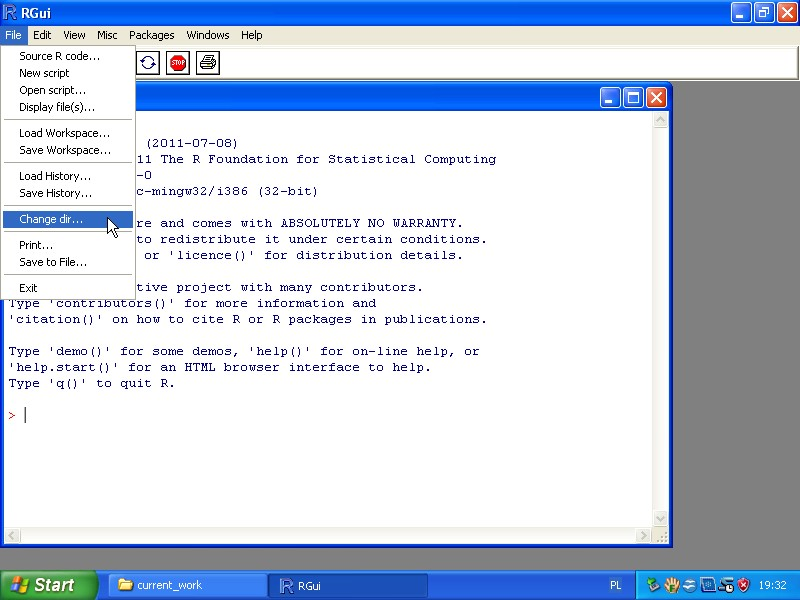
\includegraphics[width=0.65\linewidth]{img/win_setwd.jpg}
  \caption{R console on Windows: easiest way to set working directory}
\end{figure}



\subsection{Options available on GUI}

As a first step, beginners should learn how to use the graphical user
interface (GUI), which allows you to control the script's main parameters
without having to tamper with the actual code. However, if you \emph{do} 
prefer to tamper with the code, you can call the function in batch mode:
\code{stylo(gui=FALSE)}. In that case, before you start, you might
want to visit the help pages via typing the command \code{help(stylo)}.
Also, you should be familiar with additional options that can, or
rather should, be passed as arguments; they are listed on the margins
of this document.

Whenever you use the GUI, each successful execution or ``run'' of the
script will generate a \code{stylo\underscore{}config.txt} file
(saved in your working folder) which you can review (for instance,
should you have forgotten the parameters you used in your last experiment).
The parameter settings specified in this file will be retrieved at
each subsequent run of the script, so that the user won't have to
\emph{re}specify their favorite settings every time. Please note that
when you hover your cursor over the labels of each of the entries
in the GUI, tool tips will appear that will help you understand the
GUI. In the following sections we will discuss each of the different
tabs in the \code{stylo()} GUI.

No matter if you decide using GUI or not, you can pass additional
arguments from command-line. If the graphic mode is on, these ``new''
values will appear in the GUI and thus they will be still modifiable.
Some examples include:

\medskip
\code{stylo(mfw.min=300, mfw.max=300, analyzed.features="c",
ngram.size=3)}

\medskip
\code{stylo(gui=FALSE, analysis.type="MDS",
write.png.file=TRUE)}

\medskip
\code{stylo(mfw.min=100, mfw.max=1000, mfw.incr=100, analysis.type="BCT")}

\medskip



\begin{figure}
  \centering
  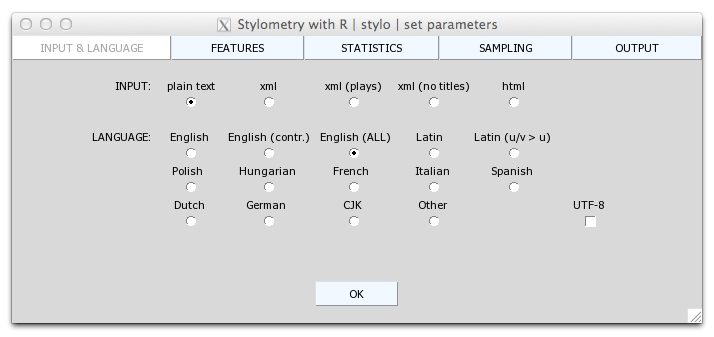
\includegraphics[width=0.8\linewidth]{img/stylo-gui_tab1.png}
  \caption{\code{stylo()} launched in its default mode: first tab on GUI}
\end{figure}



\subsubsection{Input}

This is where you specify the format of your corpus (see 4.1 above
for more details about corpus preparation, and mind possible encoding
issues). The available choices are:\margin{corpus.format=}

\begin{itemize}
  \item plain text: plain text files.\margin{"plain"} 
  
  \item xml: XML files; this option will remove all tags and TEI headers.\margin{"xml"} 
  
  \item xml (plays): XML files of plays; with this option, all tags, TEI headers,
  and speakers' names between \code{<speaker>...</speaker>} tags
  are removed.\margin{"xml.drama"} 
  
  \item xml (no titles): XML contents only: all tags, TEI headers, and chapter/section
  (sub)titles between \code{<head>...</head>} tags are removed.\margin{"xml.notitles"} 

  \item html: the option will attempt to remove HTML headers, menus, links
  and other tags.\margin{"html"} 
  
  \item UTF-8:\margin{encoding=}\margin{"UTF-8"}\margin{"native.enc"} if you use Linux or Mac, this option is immaterial; however, if your operating system is Windows, then you need to set it depending whether your dataset is encoded in Unicode (then check the option), or in ANSI (then leave it unchecked).
\end{itemize}

\subsubsection{Language}

This setting makes sure that pronoun deletion (see below) works correctly.
If you decide not to remove pronouns from your corpus (which is known
to improve authorship attribution in some languages), this setting
is immaterial (unless you are using English; see immediately below).\margin{corpus.lang=}

\begin{itemize}

\item English: this setting makes sure that contractions (such as “don’t”)
are \emph{not} treated as single words (thus ``don't'' is understood
as two separate items, “don” and “t”), and that compound words (such
as “topsy-turvy”) are \emph{not} treated as one word (thus “topsy-turvy”
becomes “topsy” and “turvy”).\margin{"English"} 

\item English (contr.): this setting makes sure that contractions (such as “don’t”) \emph{are} treated as single words (thus ``don't'' is understood as “don\^{ }t” and counted separately), but compound words (such as “topsy-turvy”) are still \emph{not} treated as one word (thus “topsy-turvy” becomes “topsy” and “turvy”).\margin{"English.contr"} 

\item English (ALL): this setting makes sure that contractions (such as
“don’t”) \emph{are} treated as single words (thus ``don't'' is understood
as “don\^{ }t” and counted separately), and that compound words (such
as “topsy-turvy”) \emph{are} treated as one word (thus “topsy-turvy”
becomes “topsy\^{ }turvy”).\margin{"English.all"} 

\item Latin: this setting makes sure that “v” and “u” are treated as discrete
character signs in Latin texts.\margin{"Latin"} 

\item Latin.corr: since some editions do not distinguish between “v” and
“u”, this option provides a consistent conversion of both characters
to “u” in each text.\margin{"Latin.corr"} 

\item CJK: Chinese, Japanese and Korean scripts, provided that the input
data is encoded in Unicode.\margin{"CJK"}

\item Other: non-Latin scripts: Hebrew, Arabic, Cyryllic, Coptic, Greek,
Georgian, Latin phonetic, so far.  Make sure your input data is in 
Unicode!\margin{"Other"}
\end{itemize}

Please do note that for all other languages, apostrophes do \emph{not}
join words and compound (hyphenated) words are split. This is not
the ideal solution and will be addressed as soon as we get to it.


\subsubsection{Features}

\begin{figure}
  \centering
  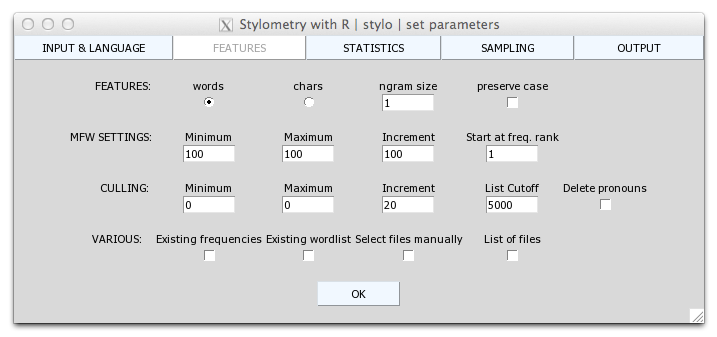
\includegraphics[width=0.8\linewidth]{img/stylo-gui_tab2.png}
  \caption{\code{stylo()} GUI, the second tab: Features, MFW Settings, Culling, Various}
\end{figure}

In many established approaches to stylometry, the (relative) frequencies
of the most frequent words (MFW) in a corpus are used as the basis
for multidimensional analyses. It has been argued, however, that other
features are also worth considering, especially word and/or character
\emph{n}-grams. The general idea behind such \emph{n}-grams is to
combine a string of individual items into a partially overlapping,
consecutive sequences of \textit{n} of these individual items. Given a sample
sentence “This is a simple example”, the character 2-grams (``bigrams'')
are as follows: “th”, “hi”, “is”, “s~”, “~i”, “is”, “s~”, “~a”, “a~”, “~s”, 
“si”, “im”, “mp”, etc. The same sentence split into bigrams
of words reads “this is”, “is a”, “a simple”, “simple example”. It
has been heavily debated in the secondary literature whether the use
of \emph{n}-grams really increases the accuracy of stylometric tests
(Hoover, 2002, 2003, 2012; Koppel et al., 2009; Stamatatos, 2009;
Eder, 2011; Alexis et al., 2014). However, it has been shown (Eder,
2013) that character \emph{n}-grams are impressively robust when one
deals with a ``dirty'' corpus (one with a high number of misspelled
characters, or one with bad {\sc ocr}). The ideal combination of parameters
in this section is another bone of contention between scholars; in
fact, Eder and Rybicki (2013) maintain that this differs not only
from language to language but also from one collection of text to
another.

\begin{itemize}
\item words: words are used as the unit. Naturally, the higher the \emph{n}
you specify, the less repetitive your n-grams there will be, and this
means poor statistics (data sparseness).\margin{analyzed.features=}\margin{"w"} 

\item characters: characters are used as the unit.\margin{"c"}

\item \emph{n}-gram size: this is where you can specify the value of \emph{n}
for your \emph{n}-grams. Certainly, setting this option to 1 makes
sure that individual words/chars will be used instead of higher-order
\emph{n}-grams.\margin{ngram.size=}\margin{<integer>}; of course,
single-letter counts do not seem like a good idea.

\item preserve case:\margin{preserve.case=}\margin{TRUE|FALSE} normally, all the words from the input texts are turned into lowercase, no matter if they are proper nouns or not -- e.g. the sentence \textit{The family of Dashwood had long been settled in sussex} will be turned into \textit{the family of dashwood had long been settled in sussex}. In some situations, however, you might be interested in preserving the case. That's the option to do it.

\item select files manually: normally, the script performs the analysis
on \emph{all} files in your \code{corpus} subfolder. If this option
is checked, a dialogue window will appear enabling the user the make
a selection of input files from the subfolder. Obviously, you can
achieve the same results by simply removing the unwanted texts from
the \code{corpus} subfolder. Again, note that this function will
expect you to select at least two different input files.\margin{[TBD]}
\end{itemize}


\subsubsection{MFW settings}

This is where you specify the size of the most-frequent-word list
that will be used for your analysis. Actually, the name is slightly
misleading, since you are not at the mercy of ``most frequent \emph{words}''
only. You can use most frequent word pairs (bigrams), character sequences,
etc. We keep the name ``MFW'' because... Well, we don't really remember
why we keep it; probably, there was no-one around to propose a better 
solution.

\begin{itemize}
\item Minimum: this setting determines how many words (or features) from
the top of the frequency list for the entire corpus will be used in
your analysis in the first (and possibly, only) run of the function.
With a value of 100 for this parameter, your analysis will be conducted
on the 100 most frequent words (features) in the entire corpus.\margin{mfw.min=}\margin{<integer>} 

\item Maximum: this setting determines how many words from the top of the
word frequency list for the entire corpus will be used in your analysis
in the last (and possibly, only) run of the function. Thus, a setting
of 1000 results in your (final) experiment being conducted on 1000
most frequent words in the entire corpus.\margin{mfw.max=\\<integer>}
(This parameter setting is especially important when working with
the bootstrap consensus trees in \code{stylo()}, a procedure which
involves running several analyses in a row. See immediately below
under ``Increment''). 

\item Increment: this setting defines the value by which the value of Minimum
will be increased at each subsequent run of your analysis until it
reaches the Maximum value. Thus, a setting of 200 (at a Minimum of
100 and a Maximum of 1000) provides for an analysis based on 100,
300, 500, 700 and 900 most frequent words.\margin{mfw.incr=}\margin{<integer>}
(As above, this parameter setting is especially important when working
with the bootstrap consensus trees in \code{stylo()}, a procedure
which involving running several analyses in a row). 

\item Start at freq. rank: sometimes you might want to skip the very top
of the frequency list\margin{start.at=}\margin{<integer>}.
With this parameter, you can specify how many words from the top of
the overall frequency rank list should be skipped. Normally, however,
users will want to set this at~1. 
\end{itemize}

N.B. For all statistical procedures (see 4.3.6 below) except the Consensus
Tree, it is advisable to set Minimum and Maximum to the same value
(this makes the Increment setting immaterial), unless you want to
produce a large series of cluster analysis, multidimensional scaling
or principal components analysis graphs in a row, for instance to
observe how/if the results change for various lengths of the MFW list.


\subsubsection{Culling}

``Culling'' refers to the automatic manipulation of the wordlist (proposed
by Hoover 2004a, 2004b). The culling values specify the degree to
which words that do not appear in all the texts of your corpus will
be removed. Thus, a culling value of 20 indicates that words that
appear in at least 20\% of the texts in the corpus will be considered
in the analysis. A culling setting of 0 means that no words will be
removed; a culling setting of 100 means that only those words will
be used in the analysis that appear in \emph{all} texts of your corpus 
at least once.

\begin{itemize}
\item Minimum: this setting specifies the first (and possibly, only) culling
setting in your analysis (cf. the minimum MFW setting).\margin{culling.min=}\margin{<integer>} 

\item Maximum: this setting specifies the last (and possibly, only) culling
setting in your analysis (cf. the maximum MFW setting)\margin{culling.max=}\margin{<integer>}.
(This parameter setting is especially important when working with
the bootstrap consensus trees in \code{stylo()}, a procedure which
involves running several analyses in a row). 

\item Increment: this defines the increment by which the value of Minimum
will be increased at each subsequent run of your analysis until it
reaches the Maximum value. Thus a setting of 20 (at a Minimum of 0
and a Maximum of 100) provides for an analysis using culling settings
of 0, 20, 30, 60, 80 and 100\margin{culling.incr=}\margin{<integer>}.
(This parameter setting is especially important when working with
the bootstrap consensus trees in \code{stylo()}, a procedure which
involves running several analyses in a row). 

\item List cutoff: Usually, it is recommended to cut off the tail of the
overall wordlist\margin{mfw.list.cutoff=}\margin{<integer>};
if you do not want to cut the list and analyze vectors of thousands
of words at once, then the variable may be set to an absurdly big
number (although this can be computationally demanding for your machine).
This setting is independent from the culling procedure. 

\item Delete pronouns: (this setting too is independent of the culling 
procedure).\margin{delete.pronouns=}\margin{TRUE|FALSE}
If this option is checked, make sure you have selected the correct
language for your corpus (see 4.3.2 above). This will select a list
of pronouns for that language inside the 
script.\margin{corpus.lang=}\margin{"English"}\margin{"Dutch"}\margin{...}
Advanced users can use this part of the tool to remove any words they
want. So far, we have pronoun lists for English, Dutch, Polish, Latin,
French, German, Spanish, Italian, and Hungarian. 
\end{itemize}

N.B. As had been mentioned above, for all statistical procedures (see
4.3.6 below) except consensus trees, it is advisable to set Minimum
and Maximum to the same value (this makes the Increment setting immaterial),
unless you want to produce a large series of cluster analysis, multidimensional
scaling or principal components analysis graphs etc. in a row.


\subsubsection{Statistics}

\begin{figure}
  \centering
  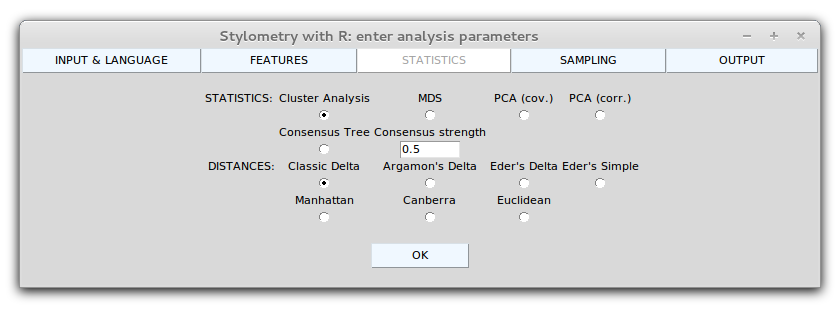
\includegraphics[width=0.8\linewidth]{img/stylo-gui_tab3.png}
  \caption{\code{stylo()} GUI, the third tab: Statistics, Distances}
\end{figure}


This is the very last moment to emphasize one important thing: the
function \code{stylo()} provides a bunch of \emph{unsupervised}
methods used in stylometry, such as principal components analysis,
multidimensional scaling or cluster analysis. The results are represented
either on a scatterplot, or a tree-like diagram (dendrogram); the
last stage of the analysis involves a human interpretation of the
generated plots.\margin{analysis.type=} The results obtained using
these techniques ``speak for themselves'', which gives a practitioner
an opportunity to notice with the naked eye any peculiarities or unexpected
behavior in the analyzed corpus. Also, given a tree-like graphical
representation of similarities between particular samples, one can
easily interpret the results in terms of finding out which group of
texts a disputable sample belongs to. On the other hand, however, these
methods cannot be \emph{validated} in terms of an automatic verification
of a given method's reliability. Thus, if you feel you'd better use
one of \emph{machine-learning} techiniques, refer to the 
funcion \code{classify()}, below.

\begin{itemize}
\item Cluster Analysis: Performs cluster analysis and produces a dendrogram,
or a graph showing hierarchical clustering of analyzed texts.
This option makes sense
if there is only a single iteration (or just a few).\margin{"CA"}
This is achieved by setting the MFW Minimum and Maximum to equal values,
and doing the same for Culling Minimum and Maximum. 

\item MDS: Multidimensional Scaling.\margin{"MDS"}
This option makes sense if there is only a single iteration (or just
a few). This is achieved by setting the MFW Minimum and Maximum to
equal values, and doing the same for Culling Minimum and Maximum. 

\item PCA (cov.): Principal Component Analysis using a covariance matrix.\margin{"PCV"}
This option makes sense if there is only a single iteration (or just
a few). This is achieved by setting the MFW Minimum and Maximum to
equal values, and doing the same for Culling Minimum and Maximum. 

\item PCA (corr.): Principal Component Analysis using a correlation matrix
(and this is possibly the more reliable option of the two, at least
for English).\margin{"PCR"} This option
makes sense if there is only a single iteration (or just a few). This
is achieved by setting the MFW Minimum and Maximum to equal values,
and doing the same for Culling Minimum and Maximum. 

\item Consensus Tree: this option will output a statistically justified
``compromise'' between a number of virtual cluster analyses results for 
a variety of MFW and Culling parameter values.\margin{"BCT"} 

\item Consensus strength: For Consensus Tree graphs, direct linkages between
two texts are made if the same link is made in a proportion of the
underlying virtual cluster analyses. The default setting of 0.5 means
that such a linkage is made if it appears in at least 50\% of the
cluster analyses.\margin{consensus.strength=}\margin{<integer>}
Legal values are $0.4-1$. This setting is immaterial for any other
Statistics settings. 
\end{itemize}


\subsubsection{Distances}

This is where the user can choose the statistical procedure used to
analyze the distances (i.e. the similarities and differences) between
the frequency patterns of individual texts in your corpus. Although
this choice is far from trivial, some of the following measures seem
to be more suitable for linguistic purposes than others. On theoretical
grounds, Euclidean Distance and Manhattan Distance should be avoided
in stylometry based on word frequencies (unless the frequencies are
normalized; see: Delta). Canberra Distance is quite troublesome but
effective e.g. for Latin; it is very sensitive to rare vocabulary,
and thus might be a good choice for inflected languages, with sparse
frequencies (it should be combined with careful culling settings and
a limited number of MFWs taken into analysis). For English, usually
Classic Delta is a good choice: mathematically speaking (Argamon,
2008), it is simply Manhattan distance applied to normalized 
(\textit{z}-scored) word frequencies. A theoretical explanation of 
the measures implemented in this function is pending. The available 
distance measures are as follows:\margin{distance.measure=}

\begin{itemize}
\item Euclidean Distance: basic and the most ``natural''.\margin{"dist.euclidean"}
It is an obvious choice when your variables are similarly distributed.
However, since word distributions are not similar at any rate (e.g.
compare the huge difference between the frequencies of ``the'' and ``dactyloscopy''),
this distance measure is not appropriate to testing vectors of dozens
of most frequent words. Or, to be precise, it could be used to assess
less frequent (content) words. According to Zipf's law, these words
are distributed more or less similarly in a corpus since, by being
less common than function words, they appear in the flattened sections
of a Zipf curve. 
\[
\delta_{(AB)}=\sqrt{\sum_{i=1}^{n}\left\vert (A_{i})^{2}-(B_{i})^{2}\right\vert }
\]



%\[ \delta_{(AB)} = \sqrt{ \sum_{i=1}^{n} %
%                     \left\vert f_{i}(A)^2 - f_{i}(B)^2 \right\vert} \]
where: \\
 $n=$ the number of MFWs (most frequent words), \\
 $A,B=$ texts being compared, \\
 $A_{i}=$ the frequency of a given word $i$ in the text $A$, \\
 $B_{i}=$ the frequency of a given word $i$ in the text $B$. \\


\item \noindent Manhattan Distance: obvious and well documented.\margin{"dist.manhattan"}
It shares the pros and cons of Euclidean Distance. 
\[
\delta_{(AB)}=\sum_{i=1}^{n}\left\vert A_{i}-B_{i}\right\vert 
\]

\item Classic Delta as introduced by Burrows (2002).\margin{"dist.delta"}
Since this measure relies on \textit{z}-scores -- i.e. normalized word frequencies
-- it is dependent on the number of texts analyzed and on a balance
between these texts: if a corpus contains, say, a large nuber of plays
by Lope de Vega and only one play by Calderón de la Barca, the final
results might by biased. 
\[
\Delta_{(AB)}=\frac{1}{n}\sum_{i=1}^{n}\left\vert \frac{A_{i}-\mu_{i}}{\sigma_{i}}-\frac{B_{i}-\mu_{i}}{\sigma_{i}}\right\vert 
\]
where: \\
 $n=$ the number of MFWs (most frequent words or other features), \\
 $A,B=$ texts being compared, \\
 $A_{i}=$ the frequency of a given feature $i$ in the text $A$, \\
 $B_{i}=$ the frequency of a given feature $i$ in the text $B$, \\
 $\mu_{i}=$ mean frequency of a given feature in the corpus, \\
 $\sigma_{i}=$ standard deviation of frequencies of a given feature.


\noindent Argamon (2008) showed that the above formula can be simplified
algebraically: 
\[
\Delta_{(AB)}=\frac{1}{n}\sum_{i=1}^{n}\left\vert \frac{A_{i}-B_{i}}{\sigma_{i}}\right\vert 
\]


\item Argamon's Linear Delta, or Euclidean distance applied to normalized
(\textit{z}-scored) word frequencies (Argamon, 2008).\margin{"dist.argamon"}
The distance is sensitive to the number of texts in a corpus. 
\[
\Delta_{(AB)}=\frac{1}{n}\sum_{i=1}^{n}\sqrt{\left\vert \frac{(A_{i})^{2}-(B_{i})^{2}}{\sigma_{i}}\right\vert }
\]

\item Eder's Delta: it is a modification of standard Burrows's distance;\margin{"dist.eder"}
it slightly increases the weights of frequent words and rescales less
frequent ones in order to suppress discriminative strength of some
random unfrequent words. The distance was meant to be used with highly
inflected languages. It is sensitive to the number of texts in a corpus.
\[
\Delta_{(AB)}=\frac{1}{n}\sum_{i=1}^{n}\left(\left\vert \frac{A_{i}-B_{i}}{\sigma_{i}}\right\vert \times\frac{n-n_{i}+1}{n}\right)
\]
where: \\
 $n_{i}=$ the position of a given feature on a frequency list (i.e. its rank).

\item Eder's Simple: a type of normalization as simple as can be (independent
on the size of the corpus), intended to convert the implications of
Zipf's law.\margin{"dist.simple"} The normalization
used in this distance is so obvious and so widely-spread in exact
sciences that naming it ``Eder's Simple Distance'' is an abuse, so to
speak. 
\[
\delta_{(AB)}=\sum_{i=1}^{n}\left\vert \sqrt{A_{i}}-\sqrt{B_{i}}\right\vert 
\]

\item Canberra Distance: sometimes amazingly good.\margin{"dist.canberra"}
It is very sensitive to differences in rare vocabulary usage among
authors. On the other hand, this can be a disadvantage, since sensitiveness
to minute differences in word occurrences also means significant sensitiveness
to noise. Last but not least, Canberra Distance is very sensitive
to the number of words (features) analyzed. 
\[
\delta_{(AB)}=\sum_{i=1}^{n}\frac{\left\vert A_{i}-B_{i}\right\vert }{\left\vert A_{i}\right\vert +\left\vert B_{i}\right\vert }
\]

\item Cosine Distance: a classical measure, introduced to this package 
quite recently.\margin{"dist.cosine"}

\[
\cos(\theta)=\frac{A\cdot B}{\|A\|\|B\|}=\frac{\sum\limits _{i=1}^{n}{A_{i}\times B_{i}}}{\sqrt{\sum\limits _{i=1}^{n}{(A_{i})^{2}}}\times\sqrt{\sum\limits _{i=1}^{n}{(A_{i})^{2}}}}
\]

\item It is also possible to use any custom distance measure. This option is 
discussed below, in the section \ref{custom_distances}.

\end{itemize}

\subsubsection{Sampling}

When the default setting of ``No sampling'' is 
checked\margin{sampling=}\margin{"no.sampling"}, each of
the texts in its entirety is treated as a single sample. The second
option, that of ``Normal sampling''\margin{"normal.sampling"}, 
performs the analysis on equal-sized
consecutive sections of each text, and the size is determined by the
setting immediately below. Eder (2015) suggests that even better attribution
results can be achieved with ``Random sampling''\margin{"random.sampling"}, 
where samples are made up of words each randomly selected from anywhere 
in the text (``bag of words'');\margin{sample.size=}\margin{<integer>} here, 
too, the sample size must be set below.

\begin{figure}
  \centering
  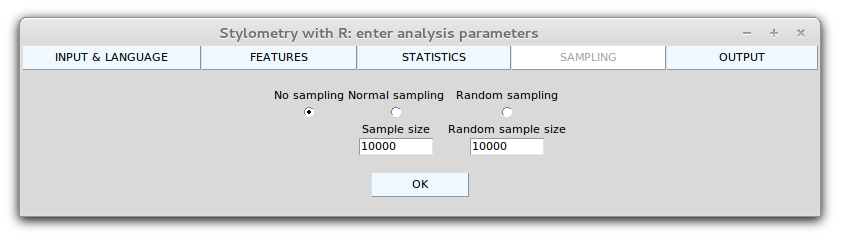
\includegraphics[width=0.8\linewidth]{img/stylo-gui_tab4.png}
  \caption{\code{stylo()} GUI, the fourth tab: Sampling}
\end{figure}


\subsubsection{Graphs}

Do you want to display the graph on the screen? Do you want to write
the graph directly to a graphics file? Which format? If you've been
thinking about any plots, these are the options to fiddle with. You
can display the graph on the screen \emph{and} write to a file (the
latter will be done with much better quality). The produced files
are saved in your working directory. As has already been mentioned,
the name of your working directory is used both as the title on top
of the graph (see 4.3.10 below) and as the name of the graph files;
some important parameter settings (for MFW list size, culling, pronoun
deletion, statistical method) are also placed on the graph and in
the name of the file. However, remember that if you perform another
analysis with the same parameters on a slightly modified corpus, this
will overwrite the earlier graph.


\begin{figure}
  \centering
  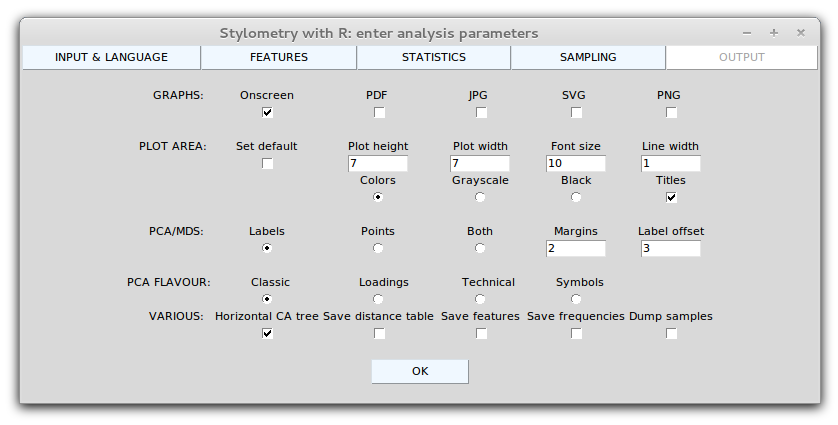
\includegraphics[width=0.8\linewidth]{img/stylo-gui_tab5.png}
  \caption{\code{stylo()} GUI, the fourth tab: Output}
\end{figure}


\begin{itemize}
\item Onscreen: check this if you want to display the graph on the screen.\margin{display.on.screen=}\margin{TRUE|FALSE} 

\item PDF: check this to obtain a PDF file with your graph.\margin{write.pdf.file=}\margin{TRUE|FALSE} 

\item JPG: check this to obtain your graph in JPEG format.\margin{write.jpg.file=}\margin{TRUE|FALSE} 

\item SVG: check this to produce a SVG vector file (XML-based scalable image
format). Useful if you want to embed your plot in HTML code, or to
edit it further with, say, Inkscape.\margin{write.svg.file=}\margin{TRUE|FALSE} 

\item PNG: check this to obtain your graph in PNG format (probably the safest
option if you want publication-ready resolution).\margin{write.png.file=}\margin{TRUE|FALSE} 
\end{itemize}

\subsubsection{Plot area}

Further graphic options. Here you can specify the dimensions of the
plot area (expressed in inches, yes, even though the makers of the
package are all honest Continental Europeans and usually think in
centimeters), font size, thickness of the lines used to plot the graphs,
etc. Since it is usually hard to remember all the values, an additional
option is provided to reset the picture options -- if this is checked,
the remaining options will be overwritten and the defaults restored.

\begin{itemize}
\item Set default: this is the above-mentioned ``amnesia button''.\margin{plot.options.reset=}\margin{TRUE|FALSE}
If you fiddle too much with different graphic settings and forget,
say, the default size of scatterplots, this option is exactly what
you need. (Remember, however, that some computers hate the ``amnesia
buttons'', HAL from \emph{2001: A Space Oddyssey} being the most convincing
caveat). 

\item Plot height: self-evident. The valid units are inches.\margin{plot.custom.height=} 

\item Plot width: self-evident. The valid units are inches.\margin{plot.custom.width=} 

\item Font size: self-evident.\margin{plot.font.size=}\margin{<integer>}
The unit is ``points'' (a detailed explanation what type of ``points''
it is and how they are related to ``typographic points'', ``Didot points'',
``Postscript points'' etc. can be skipped here; the only thing worth
noting is that they are the same ``points'' as in popular office programs,
like MS Office). 

\item Line width:\margin{plot.line.thickness=}\margin{<integer>} if
you plan to re-scale your plot, you might also want to increase the
thickness of the lines in your graph. This value is expressed in R
generic units (1~is default). 

\item Colors:\margin{colors.on.graphs=}\margin{"colors"}
when this option is checked, the script will automatically assign
the same colors to texts with the same first segment of their file
names (the first string ending in ``{}\code{\underscore}''). 

\item Grayscale:\margin{"grayscale"} select
this option to have automatic color coding (in greyscale). The file
names convention: see above. While the graphs become less pretty than
when colored, this might be your method of choice if the journal you're
planning to publish in makes you pay for color illustrations their
weight (or, rather, resolution) in gold.

\item Black:\margin{"black"} select to have
a black \& white graph. No file naming convention is required with this option. 

\item Titles:\margin{titles.on.graphs=}\margin{TRUE|FALSE} if this
is checked, the graphs will contain a main (top) title (based on the
name of your folder and your choice of the statistics option) and
a subtitle (bottom) showing the distance metric which you selected,
as well as the MFW, Culling, Feature and Consensus settings.%
\margin{custom.graph.title=}\margin{"Any text"}
If you don't want to have the title decided automatically, you need to 
pass an argument \code{custom.graph.title}.
\end{itemize}


\subsubsection{PCA/MDS}

More graphic options. The following settings, however, apply to scatterplots
only, i.e. to the plots produced by principal component analysis and
multidimensional scaling.

\begin{itemize}
\item Labels:\margin{text.id.on.graphs=}\margin{"labels"}
to identify samples on MDS/PCA plots using their labels, or names,
as specified in filenames (see 4.1 above). 

\item Points:\margin{"points"} instead of
labels, use points to show the positions of the particular samples.
This option might be helpful if you want to represent a large number
of samples on one plot. 

\item Both:\margin{"both"} in some cases,
you might be interested to get \emph{precise} positions of samples
on a graph \emph{and} to keep the samples' labels on. This option
pinpoints the exact locations of the samples using points, and slightly
offsets the labels (see the option `Label offset' immediately below). 

\item Margins:\margin{add.to.margins=}\margin{<integer>} if you use
particularly long samples' names (labels) and/or simply want to add
some blank space on your plot, set custom margin size (in percentage
of plot area). You can find out your best setting by trial and error.

\item Label offset:\margin{label.offset=}\margin{<integer>} set custom
offset between label and point (in percentage of plot area). 
\end{itemize}



\subsubsection{PCA flavour}

Even more graphic options.\margin{pca.visual.flavour=} Should you
want to use PCA, you can choose one of the four visualization flavors.

\begin{itemize}
\item Classic:\margin{"classic"} original PCA visualization using 
(colored, if applicable) sample names or points. 

\item Loadings:\margin{"loadings"} display
PCA feature (word etc.) loadings. This type of visualization is aimed
to show the discriminative strength of particular features (e.g. words)
across two first principal components. Some visual similarity to popular
``word clouds'' makes this approach attractive and comprehensive. 

\item Technical:\margin{"technical"} technical
greyscale PCA visualization, showing feature loadings as well as a
PC barplot. Potentially useful for greyscale printing in traditional
publications. 

\item Symbols:\margin{"symbols"} select to
display the samples in your PCA with a group symbol (instead of their
entire name). Potentially useful when dealing with lots of samples. 
\end{itemize}



\subsubsection{Various}

\begin{itemize}
\item Horizontal CA tree:\margin{dendrogram.lay-\\
out.horizontal=}\margin{TRUE|FALSE} select to have your cluster 
analysis graph oriented horizontally. Probably the better option for 
clarity, especially if there are a lot of samples to fit on one dendrogram. 

\item Save distance table:\margin{save.distan-\\
ce.tables=}\margin{TRUE|FALSE} save final distance table(s) in separate 
text file(s). In most cases, you will not need to use this option. 

\item Save features:\margin{save.analy-\\
zed.features=}\margin{TRUE|FALSE} save final feature (word, n-gram) 
list(s), e.g. the words actually used in the analysis. Use this option 
to have more control over the experiment: if you feel that your results 
are suspicious or too good to be true, you can open the generated file 
and check the features used. 

\item Save frequencies:\margin{save.analyzed.freqs=}\margin{TRUE|FALSE} 
this option gives you even more control: you can inspect frequencies 
of each word across the whole corpus. Switching this option saves 
frequency table(s) in separate text file(s). 

\item Dump samples:\margin{dump.samples=}\margin{TRUE|FALSE} if you
still feel that your experiment in not supervised enough, you migth
be interested in a ``post mortem'' inspection of all the samples used:
this option dumps the original samples (either whole texts, or chunks
specified using the ``Sample size'' option above) to an external file.
Be aware, however, that a corpus containig dozens of full-sized novels
might produce a huge dump file. 
\end{itemize}

\section{classify()}

This function performs a number of machine-learning algorighms of
classification: Delta (Burrows, 2002), \textit{k}-nearest neighbors,
support vectors machines, naive Bayes, and nearest shrunken centroids
(Jockers and Witten, 2010). Most of the options are derived from the
above-mentioned \code{stylo()} function.

Unlike explanatory methods as supported by \code{stylo()}, this
approach involves two stages of the analysis. In the first step, 
the traceable differences between samples produce a set of rules, 
or a classifier, for discriminating authorial ``uniqueness'' in style. 
The second step is of predictive nature -- using the trained classifier, 
the machine assigns other text samples to the authorial classes established 
by the classifier; any disputed or anonymous samples will be assigned to one 
of the classes as well, provided that such a classification is usually based 
on probabilistic grounds.

The procedure described above relies on an organized corpus of texts. 
Namely, the clue is to divide all the available texts into two groups: 
primary (training) set and secondary (test) set. The first set, being 
a collection of texts written by known authors (``candidates''), serves 
as a sub-corpus for finding the best classifier, or discrimination rules, 
while the second set is a pool of texts of known authors, anonymous texts, 
disputed ones, and so on. The better the classifier, the more samples from 
the test set are attributed (``guessed'') correctly and the more reliable 
the attribution of the disputed samples.

The function writes the resulting authorship (or similarity) candidates
to a logfile (\code{results.txt}) in the current working directory.



\subsection{Corpus preparation}

Since machine-learning methods involve two sets of texts instead of
one, you need to create two subdirectories within your working directory.
You don't really need to name this directory in any special way --
no graphs will be generated and thus no titles on graph will be used.
However, the names of both subfolders are very important: the one
containing training samples should be named \code{primary\underscore{}set},
and the test set should be titled \code{secondary\underscore{}set}
(all file names are case sensitive!). In a usual authorship attibution
study, the training set will contain at least one text by each candidate author,
preferably one ``representative'' for his/her work, whatever that is
(thus, for Goethe, something else than \emph{Farbenlehre}; for Dickens,
probably not \emph{The Pickwick Papers}). In the test set, you usually
put the anonymous or disputed samples you want to analyze, but in
most cases you also include a number of known texts to test the robustness
of a particular method. To keep the things simple: if you collect
a number of texts written by women and men in the training set, you
should also put some other text written by both groups (to provide ``unseen'' 
or ``fresh'' data) to the test set to see if they are correctly recognized.
A sample corpus of English writers might be split into two subsets
as follows:


\medskip

\code{
\noindent
\textcolor{darkgreen}{ABronte}\underscore Agnes.xml \\
\textcolor{darkred}{Austen}\underscore Emma.xml \\
\textcolor{myyellow}{Conrad}\underscore Nostromo.xml \\
\dots
}

\medskip

\code{
\noindent
\textcolor{darkgreen}{ABronte}\underscore Tenant.xml \\
\textcolor{darkred}{Austen}\underscore Pride.xml \\
\textcolor{darkred}{Austen}\underscore Northanger.xml \\
\textcolor{myyellow}{Conrad}\underscore Lord.xml \\
\textcolor{darkblue}{Dickens}\underscore Pickwick.xml \\
\textcolor[rgb]{0.3,0.3,0.3}{Anonymous}\underscore Strange-novel.xml \\
\dots
}

\medskip


The number of samples to be kept in these subfolders depends on the
method you are going to use. For Delta, support vector machines, and
\textit{k}-NN, the minimal number of texts per class is 1 (as in the above
example). Both naive Bayes and nearest shrunken centroids require
at least two samples per class to be put into the training set. (Certainly,
if you are short of texts, you can cheat: by putting a given sample
twice into the training set under two different names, e.g. \code{Swift\underscore{}Tub-1.txt},
\code{Swift\underscore{}Tub-2.txt}). However, it is a commonly
accepted fact that the more training data the better -- whenever you
have enough texts available, put a good portion of them into the training
set.

Another aspect of the above question is the nature of your stylometric
test. If you want to assess authorship, then a couple of texts per
``candidate'' should be fine, but if you want to find a rule of gender
differentiation, then you probably should collect quite a lot of textual
data written by men and women. And if you believe it is possible to
separate left-handed and right-handed writers, you need to take tons
of training texts, and even then your experiment will lack some methodological
rigour (it is sometimes called ``the risk of modeling a noise'').


\subsection{Calling the function}

The function is evoked by the command \code{classify()}.


\subsection{Options}

Most of the options are derived from the \code{stylo()} function.
Refer to the section 4.3 for further details.


\subsubsection{Options inherited from \code{stylo()}}

Input (4.3.1), Language (4.3.2), Features (4.3.3), MFW settings (4.3.4),
Culling (4.3.5), Delta Distances (4.3.7), Sampling (4.3.8), Output:
various (4.3.13).


\subsubsection{Statistics}
\begin{itemize}
\item Delta:\margin{classification.method=}\margin{"delta"}
Burrows's Delta. 

\item k-NN:\margin{"knn"} \textit{k}-nearest neighbor
classification. 

\item SVM:\margin{"svm"} support vector machines. 

\item NaiveBayes:\margin{"naivebayes"} naive
Bayes classification. To use this method, you should have at least
two texts of each class (author, genre, etc.) in the primary (training)
set. 

\item NSC:\margin{"nsc"} nearest shrunken
centroid classification. To use this method, you should have at least
two texts of each class (author, genre, etc.) in the primary (training)
set. 
\end{itemize}

\subsubsection{General}
\begin{itemize}
\item ALL culling:\margin{culling.of.all.}\margin{samples=}\margin{"TRUE|FALSE"}
the culling procedure (cf. 4.3.5) is based on the percentage of samples 
containing a given word. To compute this ratio, one might want to use the 
texts from the first set only, or from both sets. 

\item ALL wordlists:\margin{reference.wordlist.}\margin{of.all.samples=}\margin{"TRUE|FALSE"}
the both tables of frequencies are build using the pre-prepared word
list of the whole primary set (default). Alternatively, one might
want to prepare this list of both sets by activating this option. 

\item ALL z-scores:\margin{z.scores.of.all. samples=}\margin{"TRUE|FALSE"}:
how the \textit{z}-scores should be calculated. If the variable is set to FALSE,
the \textit{z}-scores are relying on the primary set only (this should be better
in most cases; after all, this is the classical solution used by Burrows
and Hoover). Otherwise, the scaling is based on all the values in
the primary and the secondary sets. (This option is applicable to
Delta only). 
\end{itemize}

\subsubsection{SVM options}

Support vector machines classification settings: refer to \code{help(svm)}
from \code{library(e1071)} for details.
\begin{itemize}
\item Linear:\margin{svm.kernel=}\margin{"linear"}
linear kernel of SVM; probably the best choice in stylometry, since
the number of variables (e.g. MFWs) is many times bigger than the
number of classes. 
\item Polynomial:\margin{"polymonial"} polynomial
kernel of SVM. 
\item Radial:\margin{"radial"} radial kernel
of SVM. 
\item Degree:\margin{svm.degree=}\margin{<integer>} parameter needed
for kernel of type ``polynomial'' (default: 3). 
\item Coef0:\margin{svm.coef0=}\margin{<integer>} parameter needed
for kernel of type ``polynomial'' (default: 0). 
\item Cost:\margin{svm.cost=}\margin{<integer>} cost of constraints
violation (default: 1); it is the C-constant of the regularization
term in the Lagrange formulation. 
\end{itemize}

\subsubsection{k-NN options}
\begin{itemize}
\item k value:\margin{k.value=}\margin{<integer>} the \textit{k} value
in \textit{k}-Nearest Neighbour algorithm, or number of neighbours
to be considered. Certainly, the bigger the number the better the
performance, but, on the other hand, to set this value to 3, you need
to have at least three samples per class in the training set. If you
keep just one text per class in the training set, the performance
is \textit{ex definitione} suboptimal. 
\item l value:\margin{l.value=}\margin{<integer>} minimum vote for
definite decision, otherwise ``doubt''. (More precisely, less than
$k-l$ dissenting votes are allowed, even if $k$ is increased by
ties). 
\end{itemize}

\subsubsection{Output: general}
\begin{itemize}
\item Misclassifications:\margin{final.ranking.of.}\margin{candidates=}\margin{TRUE|FALSE}
here you can specify whether you want to list the misclassified samples
into the log file. Certainly, in most cases you will want to have
them listed. However, if you plan to perform a multi-iterated large-scale
experiment to test performance of a given method, you will probably
prefer to switch off all that verbosity. 
\item Count good guesses:\margin{how.many.correct.}\margin{attributions=}\margin{TRUE|FALSE}
report the number of correct guesses for each iteration (written to
the log file). To say the truth, this option is a bit obsolete, since
using \code{classify()} you are almost always interested in the
number of correctly classified samples. 
\item No. of candidates:\margin{number.of.candidates=}\margin{<integer>}
final ranking of candidates is directed to a file. You may specify
the number of final ranking candidates to be displayed (at least 1).
This option works for Delta only. 
\end{itemize}

\section{rolling.delta(), rolling.classify()}

The procedure “Rolling Delta”, supported by the function \code{rolling.delta()}
is reminiscent of a number of earlier applications of the metric (e.g.
van Dalen-Oskam and van Zundert, 2007; Kestemont, 2010; Burrows, 2010).
The general goal is to use the Delta metric to reliably visualize
stylistic shifts in texts, for instance in order to study the stylistic
evolution in texts, to detect plagiarism or to pinpoint authorial
takeovers in the case of collaborative authorship.

The first step involves a “windowing” procedure in which each reference
text is segmented into consecutive, equal-sized samples or ``windows''
(\code{window.size} parameter). The samples are allowed to partially
overlap (\code{step.size} parameter). If we specify a \code{window.size}
of 5,000 and a \code{step.size} of 100, for example, the first
sample of a text contains words 1--5,000, the second 101--5,100, the
third sample 201--5,200, and so forth (see 6.3.2 below). Like Delta,
our procedure uses the relative frequencies of a (preferably small)
set of \textit{n} words which were most frequent in the entire collection of
reference texts. Subsequently, we compute a representative centroid
for each reference text that consists of the mean relative frequency
for each of the \textit{n} words in the windows extracted from the text,
as well as the standard deviation.

We then proceed to the analysis of the test text. We divide it into
windows too and iteratively compute the difference in style (the Delta)
between each test window and each reference centroid. In order to
calculate the Delta with the $n$ most frequent words we employ the following
formula. Let $C$ be an author’s centroid and let $W$ be the window we
wish to compare it to. For each of the $n$ words, we calculate the absolute
difference between its average frequency in $C$ and its frequency in
$W$. Next, we weigh this difference using each word’s standard deviation
in the centroid. (Words whose frequencies display significant fluctuation
in a reference text’s windows are thus assigned a lower weight.) The
final Delta is the summation of these $n$ weighted differences.

\[
\Delta(C,W)=\sum_{i=1}^{n}\frac{1}{\sigma_{i}C}\vert\mu_{i}(C)-f_{i}(W)\vert
\]


After “rolling” through the test text we can plot the resulting series
of Deltas for each reference text in a graph. The relatively lower
the Deltas for a given reference text, the relatively more similar
the style in the test windows – and vice versa (cf. Hoover, 2004b:
471). If the curve for a text would show a sudden drop at a given
position, this could be indicative of a stylistic change in the text
(which might, for instance, be caused by one author taking over from
another. One can use vertical lines in the plot to mark the position
of certain events in the test text as an aid in interpreting the graph
(e.g. chapter beginnings).


\subsection{Corpus preparation}

You will need two subfolders in your working directory: \code{primary\underscore{}set}
should contain the test texts: the individual writings by each of
the authors who collaborated on the test text -- the latter goes into
the \code{secondary\underscore{}set} subfolder (once again, the names are case-sensitive).
In the pilot study for this method (Rybicki et al., 2014), the primary
set was composed of individual writings by Joseph Conrad and individual
writings by Ford Madox Ford, such as, respectively, \emph{The Heart
of Darkness} and \emph{The Good Soldier}; the secondary set only contained
a single text at a time: one of the texts written in collaboration
by the two writers, such as \emph{The Inheritors}. To study another
Conrad/Madox collaboration, \emph{The Inheritors} had to be removed
from the secondary set and replaced by, say, \emph{Romance}.


\subsection{Calling the function}

The function is evoked by the command \code{rolling.delta()}.


\subsection{Options}

While many of the options are derived from the main \code{stylo()} function
-- especially in the ``Input \& Language'', ``Statistics'', and
``Output'' tabs, some differences must be emphasized here.


\subsubsection{Features}

Contrarily to this section in \code{stylo()}, MFW settings only
use a single value (Maximum) since only one analysis is performed,
and the same is true of the Culling value.


\subsubsection{Sampling}

The ``Slice length'' parameter sets the size of the text ``window''
or of consecutive samples cut out one by one from the test text. ``Stepsize''
controls the size of the overlap between two consecutive windows.
For the default settings, a slice length of 5,000 and a stepsize of
1,000 takes the first 5,000 words from the beginning of the test text
as the first sample, the section from the 1001th word in the text
to its 6,000th word, and so forth. Beware of very small stepsize values:
we have not yet seen a computer that would not hang R at a setting
of 1!


\subsubsection{Colors}

An additional tab has been added to control the colors of the curves
for each training set text. Two courses of action are advisable here.
If you only want to differentiate the texts by author, you might want
to set a single color from the pull-down fields for that author's
texts, and another for the texts by the second writer. ``Color~1''
sets the color for the text that comes first alphabetically in the
ordinary listing of filenames, ``Color~2'' colors the second text,
etc. Thus, to use the above examples, all texts by Conrad would precede
those by Ford, and \code{conrad\underscore{}heart.txt} (for \emph{The Heart of
Darkness}) would precede \code{conrad\underscore{}jim.txt} (for \emph{Lord Jim}),
etc. The other alternative is to use different shades of the same
basic color for each writer so that the similarity between the particular
sets can be more visible. The colours in the pull-down fields can
be replaced with other text names of colors in R's pallette; you can
get a listing of these by invoking R's \code{colors()} command.


\section{oppose()}

It performs a contrastive analysis between two given sets of texts,
using Burrows's Zeta (2007) in its different flavors, including Craig's
extensions (Craig and Kinney, 2009). Also, the Whitney-Wilcoxon procedure
as introduced by Kilgariff (2001) is available. The function generates
a vector of words significantly \textit{preferred} by a tested author, and
another vector containing the words significantly \textit{avoided}.


\subsection{Corpus preparation}

Suppose you want to find out the characteristic words of men and women,
and then to see which of the anonymous books in a corpus might have
been written by men, and which by women. In order to do this, you
put all the women into the \code{primary\underscore{}set} subfolder
of your working directory, and all the men into the \code{secondary\underscore{}set}
folder, and then you place the anonymous texts in the \code{test\underscore{}set}
subfolder (the \code{test\underscore{}set} folder is optional;
the script \textit{will} run if it is not there or if you are not interested
in the anonymous texts).


\subsection{Calling the function}

The function is evoked by the command \code{oppose()}.


\subsection{Options}

\begin{itemize}
\item Text slice length (in words), the default is 10,000 words. This parameter
refers to the size of the samples into which each text is ``sliced''
in order to perform zeta. 

\item Text slice overlap (in words). The default, 0, means that the first
sample will contain words 1 to 10,000 in the text, the second sample
10,001 to 20,000, etc. If you set it to 2000, the first sample will
contain words 1 to 10,000 in the text, the second sample 8001 to 18,000,
etc. Beware of low values: setting it to 1 will result in a huge number
of samples and R might eventually crash. 

\item Rare occurrences threshold: the default, 2 prevents hapax legomena
and dislegomena from appearing in the resulting zeta wordlist file;
1 gets rid of just hapax legomena, 10 makes sure only words that appear
at least 11 times in the corpus are included in the list. 
\item Filter threshold (default 0.1) gets rid of word of weak discrimination
strength (it's like \emph{p}, the degree of statistical significance,
in various standard statistical texts). The higher the number, the
less words appear in the final wordlist. It does not normally exceed
0.5. To quote Maciej Eder: ``if the `craig.zeta' method is selected,
you might probably want to filter out some words of weak discrimination
strength. Provided that 2 means the strongest positive difference
and 0 the strongest negative difference (Hoover, 2009), the values
either just above or just below 1 are not significant and thus can
be (or rather should be) omitted. If chisquare method was chosen,
all the differences of $p$ value below 0.05 were filtered out, in pure
Zeta, there is no a priori solution. Threshold 0.5 would filter out
a vast majority of words, threshold set to 1 would filter all the
words in a corpus.'' 

\item Method: we have 3 zeta flavors so far: Craig's (as described by him
and Hoover); Eder's (not documented yet, but basically derived from 
Canbera distance measure); chi-square (not documented yet). 

\item Output: self-evident, except that ``Identify
points'' only works (if it \textit{does} work) with output set
to ``Onscreen''.
\end{itemize}

The script outputs two files: a list of \code{words\underscore{}preferred.txt},
which are words significantly \textit{preferred} by the primary author(s);
and a list of \code{words\underscore{}avoided.txt}, which are
words significantly \textit{avoided} by the primary author(s).

The graph plots the frequencies of both word categories, preferred
in avoided, for each sample into which the texts have been sliced;
normally, primary set samples (marked as circles; colors correspond
to the authors of the texts from which they were taken) should appear
in the top left corner of the plot (high words preferred frequencies,
low words avoided frequencies), while the secondary set samples (marked
as triangles) should gather in the bottom right (low words preferred
frequencies, high words avoided frequencies). Samples from texts by
authors in the test set are marked as crosses; if they overlap with
either the primary or the secondary set samples, this shows the stylistic
similarity. Also, a polygon marking the outside limit of the primary
set samples, and another one for the secondary set, are drawn on the
graph. Of course, you can now combine the words preferred and avoided 
files into a single \code{wordlist.txt} file and use the \code{stylo()} 
function for better discrimination between two groups of texts.

\section{Options unavailable on GUI}

\subsection{Cluster analysis linkage}

\begin{itemize}
\item linkage:\margin{linkage=} algorithm for establishing clusters in a dendrogram;  choose one of the following linkage methods: \code{"nj"}, \code{"ward"} (default), \code{"single"}, \code{"complete"}, \code{"average"},  \code{"mcquitty"}, \code{"median"}, \code{"centroid"}.
\end{itemize}

\subsection{Network analysis support}

The package ``stylo'' does not produce any networks {\it per se}, however, 
it does generate tables of edges/nodes (or, edges alone), using two Eder's 
algorightms of establishing connections between the nodes (Eder, forthcoming). 
The table can be loaded into Gephi (https://gephi.org). To get such a table, 
invoke the function \code{stylo()} with an argument \code{network=TRUE}, 
and optionally with some other arguments, as listed below. E.g.:


\medskip
\code{stylo(network=TRUE, network.type="undirected")}


\begin{itemize}

\item network:\margin{network=}\margin{TRUE|FALSE} an output file (or files) will be generated when this option 
is set TRUE, if this is set FALSE, the options immediately below are 
immaterial. (Default: FALSE).

\item network.tables:\margin{network.tables=}\margin{"edges"}\margin{"both"} one of two flavors of output: either one table (edges),  or two (edges and nodes). Choose ``edges'' (default), or ``both'', respectively. Using both tables instead of one allows you to edit the table of nodes in, say, Excel, in order to set some node attributes. When you use two  tables, however, make sure you import edges to Gephi first; also, make sure you uncheck (in Gephi) the option for creating missing nodes.

\item network.type:\margin{network.type=}\margin{"undirected"}\margin{"directed"} when ``undirected'' type of network is chosen (default), then the connections \textit{from} and \textit{to} are counted together (summed into one stronger connection). When \code{"directed"} network is chosen, then the incoming connections and the outcoming ones are counted separately.

\item linked.neighbors:\margin{linked.neighbors=}\margin{<integer>} if this value is set to 1, then a link between a given sample and its nearest neighbor is established; when it is set to 2, two neighbors are connected (the nearest neighbor and the firs runner-up), etc. Default value is 3, which means that the nearest neighbor and two runners-up are taken into consideration.

\item edge.weights:\margin{edge.weights=} the connections' weights are always differentiated: the nearest neighbor has the strongest link, then comes the first runner-up, and so forth.\margin{"linear"}\margin{"quadratic"}\margin{"log"} The assigned weights might be \code{"linear"} $= 1, 2, 3, \dots, n$; \code{"quadratic"} $= 1, 4, 9, ..., n^2$; or \code{"log"} (logarithmic) $= \log(1+(1, 2, 3, ..., n))$.

\end{itemize}

\begin{figure}
  \centering
  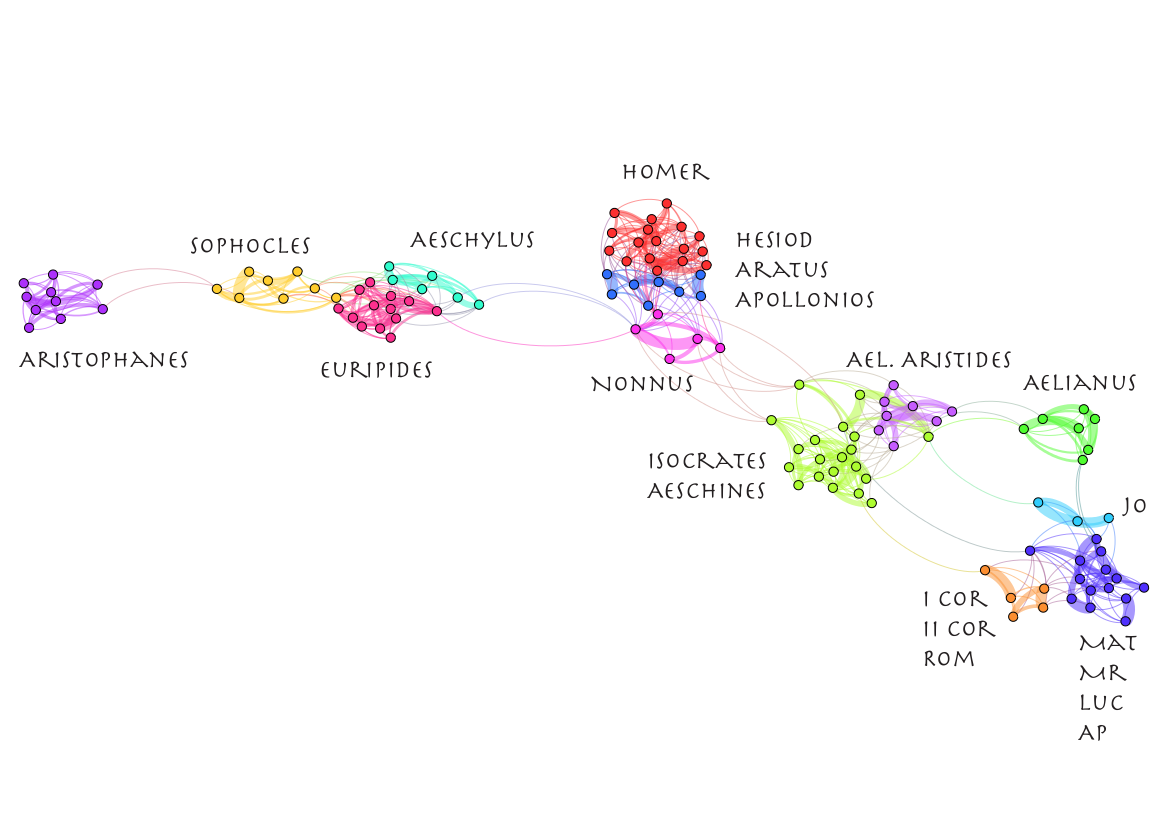
\includegraphics[width=0.8\linewidth]{img/124_Greek_texts.png}
  \caption{124 Greek texts represented as connected nodes of a network}
\end{figure}

Network analysis plots might be useful for visualizing textual relations 
in large datasets. Particular texts can be represented as nodes of a network, 
and their explicit relations as links between these nodes (Fig. 8). 
The procedure of linking is twofold (details: Eder, forthcoming). 
One of the involved algorithms computes the distances between analyzed texts, 
and establishes, for every single node, a strong connection to its nearest 
neighbor (i.e. the most similar text), and weaker connections to the 1st and 
the 2nd runner-up (i.e. two texts that get ranked immediately after the 
nearest neighbor). The second algorithm performs a large number of tests 
for similarity with different number of features to be analyzed 
(e.g. 100, 200, 300, ..., 1,000 MFWs). Finally, all the connections produced 
in particular “snapshots” are added, resulting in a consensus network. 





\subsection{Undocumented arguments}

\begin{itemize}

\item \code{features}
\item \code{frequencies}
\item \code{training.frequencies}
\item \code{test.frequencies}
\item \code{parsed.corpus}
\item \code{training.corpus}
\item \code{test.corpus}
\item \code{cv}
\item \code{cv.folds}
\item \code{encoding}
\item \code{relative.frequencies}
\end{itemize}



\section{Advanced topics}





\subsection{Batch mode}

As mentioned somewhere in this document, it is possible to pass input data into \code{stylo()} and \code{classify()} from inside R, without relying on any external files. Also, the final results -- apart from being plotted on screen and saved to the hard-drive -- are accessible as R objects. One can imagine a very complex stylometric experiment computed remotely on a high-performance server without any file reading/writing involved. The next sections provide an outline of such a pipeline design.

The datasets that can be piped into \code{stylo()} and \code{classify()} from other R functions include: (1) pre-processed corpus, in terms of a list containing vectors of words (or other countable units); see \code{help(load.corpus.and.parse)} for further details, see also an example discussed in \code{help(stylo)}, (2) table of word frequencies: an R matrix or data frame with variables (words) formatted vertically as colums, and samples (texts) ordered horizontally as rows, (3) words (MFWs) or other features to be analyzed: an R vector containing the features as elements. In the case of \code{classify()}, two corpora and/or two frequency tables are piped instead. The following executable toy example, quoted after \code{help(classify)}, shows how the training and the test corpus should be passed in a pipelne:

\begin{alltt}
     # preparing a training corpus
     txt1 = c("now", "i", "am", "alone", "o", "what", "a", "slave", "am", "i")
     txt2 = c("what", "do", "you", "read", "my", "lord")
     corpusTRAIN = list(txt1, txt2)
     names(corpusTRAIN) = c("hamlet_sample1", "polonius_sample1")

     # preparing a test corpus
     txt4 = c("to", "be", "or", "not", "to", "be")
     txt5 = c("though", "this", "be", "madness", "yet", "there", "is", "method")
     txt6 = c("the", "rest", "is", "silence")
     corpusTEST = list(txt4, txt5, txt6)
     names(corpusTEST) = c("hamlet_sample2", "polonius_sample2", 
              "uncertain_1")

     # launching the classification
     classify(training.corpus = setTRAIN, test.corpus = setTEST)
\end{alltt}

One can pass the features to be analyzed (e.g. MFWs) into \code{stylo()} or \code{classify} in a similar way. Consider the following example:

\begin{alltt}
     my.selection.of.function.words = c("the", "and", "of", "in", "if", 
                "into", "within", "on", "upon", "since")
     stylo(features = my.selection.of.function.words)
\end{alltt}

In any attempts to use existing tables of frequencies, one needs to remember that R in general, and the package \code{stylo} in particular, accepts tabular datasets with variables stored as \textit{columns}. Certainly, this might be slightly confusing, since in other statistical programs the variables are usually stored in \textit{rows}. If your dataset is formatted as follows:

\begin{center}
\begin{tabular}{c|cccccc}
 & ABronte & Austen & CBronte & Conrad & Dickens &  \\
 & {\it Agnes} & {\it Emma} & {\it Jane} & {\it Lord} & {\it Bleak} & $\dots$\\
\hline
“the”	& 4.57	& 4.24	& 4.25	& 4.19	& 4.47  & $\dots$\\
“to”	& 3.11	& 3.29	& 3.43	& 3.14	& 3.71  & $\dots$\\
“and”	& 3.19	& 3	    & 3.08	& 2.85	& 2.81  & $\dots$\\
“of”	& 2.6	& 3	    & 2.63	& 2.43	& 2.86  & $\dots$\\
“I”    & 2.17	& 2.2	& 2.13	& 2.42	& 2.22  & $\dots$\\
“a”    & 2.24	& 1.92	& 1.92	& 2.21	& 1.92  & $\dots$\\
$\vdots$ & $\vdots$ & $\vdots$ & $\vdots$ & $\vdots$ & 
$\vdots$ & $\ddots$ 
\end{tabular}
\end{center}

\noindent
then you should do a tiny tweak before piping it further:

\begin{alltt}
    my.rotated.dataset = t(my.dataset)
    stylo(frequencies = my.rotated.dataset)
\end{alltt}

\noindent
For the sake of compatibility, the tables produced by the package \code{stylo} are always saved in the transposed format -- do not be confused, then.

When it comes to the final results stored as R objects, you should remember that each function returns its value after evaluation. The main functions of the package \code{stylo} do not clutter your screen with thousands of values, but the results are there anyway. They are made invisible. To have an access to these values, pipe the function, say, \code{classify} to a variable:

\begin{alltt}
    my.results = classify()
\end{alltt}

The variable \code{my.results} is a list containing a number of elements, including tables of frequencies, classification results, and so forth. E.g. type \code{my.results\symbol{36}frequencies.training.set} to get one of the tables.

Now, since the functions accept R objects as input data, and at the same time their output is stored in R's memory as a list of R objects, it is possible to connect two functions ``on the fly''. Consider an experiment involving the function \code{oppose()}, aimed at extracting the most characteristic words for subcorpora \textit{A} and \textit{B}, which will be later used to perform a cluster analysis on some other samples. The solution is straightforward:

\begin{alltt}
    # launching `oppose' to extract significant words
    zeta.test.results = oppose()

    # combining two lists of words into one vector
    set1 = zeta.test.results\symbol{36}words.preferred
    set2 = zeta.test.results\symbol{36}words.avoided    
    words.from.zeta = c(set1, set2)

    # using the above vector as features for `stylo'
    stylo(features = words.from.zeta)
\end{alltt}


\subsection{Custom splitting rule}

When calling stylo, users can define their tokenization rules. The argument \code{splitting.rule} takes the form of a regular expression which will be used to split input character strings into discrete units, usually words. In obsolete versions of the package ‘stylo’, the default splitting sequence of chars was \code{"[\^{}[:alpha:]]+"} on Mac/Linux, and \code{"\symbol{92}\symbol{92}W+\underscore"} on Windows. Two different splitting rules were used, because regular expressions are not entirely platform-independent. In the version 0.5.6, then, assumed letter characters have been indicated explicitly. Type \code{help(txt.to.words)} to see the actual chararacter codes that were used as default rule.

If you are sure that your corpus contains clean spaces as word delimiters (i.e. there is no punctuation), you can use a very simple splitting rule, such as the one listed below. Even better, the rule might allow spaces, tab characters and newlines as word delimiters (the second variant):

\begin{alltt}
    classify(splitting.rule="[:space:]+")
    classify(splitting.rule="[ \symbol{92}t\symbol{92}n]+")
\end{alltt}

\noindent
Some other regular expressions may include:

\begin{alltt}
    "[\^{}\symbol{92}u0041-{}\symbol{92}u005A\symbol{92}u0061-\symbol{92}u007A]+"               # (standard Latin-1)
    "[\^{}\symbol{92}u00C0-\symbol{92}u00D6\symbol{92}u00D8-\symbol{92}u00F6\symbol{92}u00F8-\symbol{92}u00FF]+"  # (Western European)
    "[\^{}\symbol{92}u0100-\symbol{92}u017F]+"                            # (Central European)
\end{alltt}

\noindent
The custom splitting rule option can be also used if your input ``texts'' contain sequences of POS-tags rather than words, e.g.:

\begin{alltt}
    N-voc ADJ N-gen N-gen N-nom N-gen ADJ-NUM ABBR N-nom ADJ ...
\end{alltt}

\noindent
Then your splitting rule might look as follows:

\begin{alltt}
    "[\^{}[A-Za-z]-]+"
\end{alltt}




\subsection{Splitting rule and batch mode combined}

In many cases, the default functionalities provided by the 
library \code{stylo} can turn out to be insufficient for your needs. 
Then, you can prepare your own corpus using some of the functions provided 
by the library, then pipe it into other R functions and/or packages, and 
take it back to \code{stylo} after relevant modifications. Let's consider 
the following example in which the aforementioned custom regular expression 
solution was used. Suppose there is a collection of texts stored in a 
subdirectory "corpus". However, these texts are tagged:

\begin{alltt}
    All_NNP true_JJ histories_NNS contain_VBP instruction_NN ;_: though_RB 
    ,_, in_IN some_DT ,_, the_DT treasure_NN may_MD be_VB hard_JJ to_TO 
    find_VB ,_, and_CC when_WRB found_VBN ,_, ...
\end{alltt}

Suppose one wants do drop the lemmas and to get tags only: NNP JJ NNS VBP 
NN RB IN DT DT NN MD VB JJ TO VB CC WRB VBN RB... It is possible to 
extract the grammatical annotation via the function \code{parse.pos.tags()},
using the following code:

\begin{alltt}
    # loading all input texts from the directory `corpus':
    my.raw.data = load.corpus(files = dir(), corpus.dir = "corpus")
    
    # we invoke the function `parse.pos.tags'
    my.cool.data = parse.pos.tags(my.raw.data, tagger = "stanford", 
          feature = "pos")

    # now, we launch stylo() with an argument:
    stylo(parsed.corpus = my.cool.data)
\end{alltt}

The above function is not supported by the older versions of \code{stylo}
(ver. <0.6.2), but it can be easily worked around:

\begin{alltt}
    # loading all input texts from the directory `corpus':
    my.raw.data = load.corpus(files = dir(), corpus.dir = "corpus")

    # now, it's time for some substitutions and regular expressions:
    my.slightly.better.data = lapply(my.raw.data, gsub, 
              pattern = "[[:alpha:],.;'-]+_", replacement="")
    
    # to get rid of punctuation marks, another regexp might be helpful:
    my.acceptable.data = lapply(my.slightly.better.data, gsub,
              pattern = "[[:punct:]]+", replacement = "")
    
    # next, using the function `txt.to.words' (from the "stylo" package)
    # one can tokenize the whole corpus:
    my.cool.data = lapply(my.acceptable.data, txt.to.words)

    # the last stage is to launch the stylo() function with an argument:
    stylo(parsed.corpus = my.cool.data)
\end{alltt}

Similarly, custom tables of frequencies can be build separately, and used 
in a form of external R objects piped into \code{stylo()}:

\begin{alltt}
   # external frequencies:
   my.table = make.table.of.frequencies(my.cool.data, words = c("nn",
         "jj","dt","prp") )
   stylo(frequencies = my.table)
\end{alltt}


\subsection{Custom similarity measures}\label{custom_distances}

The package \code{stylo} in ver. >0.6.0 provides a socket for defining and 
plugging in custom distance measures. Suppose you want to test the 
Cosine Delta (or, W\"urzburg Delta) distance discussed by Jannidis, Sch\"och 
and Pielstrom (2015). Their measures is basically a regular Cosine Distance 
applied to \textit{z}-scored data. To use it with \code{stylo}, one has to
prepare a custom function that will compute the distance out of table
of frequencies. The following function does the job, even if it could be 
slighlty optimized:


\begin{alltt}
    wurzburg.cosine = function(x){
            # z-scoring the input matrix of frequencies
            x = scale(x)
            # computing cosine dissimilarity
            y = as.dist( x %*% t(x) / (sqrt(rowSums(x^2) %*% t(rowSums(x^2)))) ) 
            # then, turning it into cosine similarity
            z = 1 - y
            # getting the results
            return(z)
    }
\end{alltt}

Now, the code has to be typed (or copy-pasted) to the R console so that it 
is visible for other functions. We are ready to use the usual functions,
supplemented with an additional argument:

\begin{alltt}
stylo(distance.measure = "wurzburg.cosine")

classify(distance.measure = "wurzburg.cosine")

rolling.classify(distance.measure = "wurzburg.cosine")
\end{alltt}

Other possible applications include e.g. testing if the Entropy Distance 
outperforms other similarity measures. The code for the similarity function
is straightforward:

\begin{alltt}
    dist.entropy = function(x) {
            A = t(t(x + 1) / colSums(x + 1))
            B = t(t(log(x + 2)) / -(colSums(A * log(A))))
            y = dist(B, method="manhattan")
            return(y)
    }

stylo(distance.measure = "dist.entropy")
\end{alltt}

Etc. etc. The are plethora of possible distance measures. The users are 
encouraged to examine them all!

\subsection{Large-scale stylometric tests}


Suppose that one wants to conduct a large experiment: the goal is to perform multiple runs with different lengths of the wordlist, increasing gradually the `start.at' variable. This option is not implemented in the package \code{stylo}. However, using the batch mode it is just a few steps to success. Consider the following tailored script:

\begin{alltt}
### the script begins ###
library(stylo)

# assume we want to perform a series of tests using 50 words
# and gradually moving the starting point on the wordlist
# e.g., from 100 to 1000 by 50 (i.e. for 100, 150, 200, 250, ... 1000)
# this is a vector of the start points we want to test:
where.to.start = seq(100,1000,50)

for(current.start.point in where.to.start) \{ 

    #############
    # CORE CODE:
    # in each iteration, `stylo' will be launched in batch mode
    # the option "start.at" will be incremented
    stylo(gui = FALSE,
          display.on.screen = FALSE,
          use.existing.freq.tables = TRUE,
          corpus.lang = "English.all",
          mfw.min = 50, mfw.max = 50,
          start.at = current.start.point) 
    #############

  # now, we want to get the table of distances
  current.results = results.stylo\symbol{36}distance.table

  # what about saving this table?
  # first, we have to create a unique file name to prevent overwriting
  # the same file in each iteration:
  current.filename = paste("distances_starting_at_",
                       current.start.point, ".txt", sep="")
                       
  # now, it's time to save the results in their files
  write.table(file = current.filename, current.results)
\}

# a short message on screen, followed by a newline char:
cat("what about another stylometric test?\symbol{92}n")
### the script is done ###
\end{alltt}






\section{Error messages and troubleshooting}

[TBD]


\section*{References}

\addcontentsline{toc}{section}{References}

\indent

Alexis, A., Craig, H., and Elliot, J. (2014). Language chunking, data
sparseness, and the value of a long marker list: explorations with
word n-grams and authorial attribution. \textit{Literary and Linguistic
Computing}, \textbf{29}(2): 147--63.

Argamon, S. (2008). Interpreting Burrows’s delta: geometric and probabilistic
foundations. \textit{Literary and Linguistic Computing}, \textbf{23}(2):
131--47.

Burrows, J. (2002). Delta: a measure of stylistic difference and a
guide to likely authorship. \textit{Literary and Linguistic Computing},
\textbf{17}(3): 267--87.

Burrows, J. F. (2007). All the way through: testing for authorship
in different frequency strata. \textit{Literary and Linguistic Computing},
\textbf{22}(1): 27--48.

Burrows, J. (2010). Never say always again: reflections on the numbers
game. In McCarty, W. (ed), \textit{Text and Genre in Reconstruction.
Effects of Digitalization on Ideas, behaviors, Products and Institutions}.
Cambridge: Open Book Publishers, pp. 13--36.

Craig, H. and Kinney, A. F., eds. (2009). \textit{Shakespeare, Computers,
and the Mystery of Authorship}. Cambridge: Cambridge University Press.

van Dalen-Oskam, K. and van Zundert, J. (2007). Delta for Middle Dutch:
author and copyist distinction in Walewein. \textit{Literary and Linguistic
Computing}, \textbf{22}: 345–62.

Eder, M. (2011). Style-markers in authorship attribution: a cross-language
study of the authorial fingerprint. \textit{Studies in Polish Linguistics},
\textbf{6}: 99--114. \url{http://www.wuj.pl/page,art,artid,1923.html}.

Eder, M. (2013). Mind your corpus: systematic errors in authorship
attribution. \textit{Literary and Linguistic Computing}, 
\textbf{28}(4): 603--14.

Eder, M. (2015). Does size matter? Authorship attribution, short samples,
big problem. \textit{Digital Scholarship in the Humanities}, \textbf{30}(2):
167--82.

Eder, M. (forthcoming). Visualization in stylometry: cluster analysis 
using networks. \textit{Digital Scholarship in the Humanities}, 
\textbf{30}, doi: 10.1093/llc/fqv061, in press.

Eder, M. and Rybicki, J. (2011). Stylometry with R. In \textit{Digital
Humanities 2011: Conference abstracts}. Stanford University, CA, pp.
308--11.

Eder, M., Kestemont, M. and Rybicki, J. (2013). Stylometry with R: a suite 
of tools. In \textit{Digital Humanities 2013: Conference Abstracts}. 
Lincoln: University of Nebraska-Lincoln, pp. 487--89.

Hoover, D. L. (2002). Frequent word sequences and statistical stylistics.
\textit{Literary and Linguistic Computing}, \textbf{17}: 157--80.

Hoover, D. L. (2003). Frequent collocations and authorial style. 
\textit{Literary and Linguistic Computing}, \textbf{18}: 261--86.

Hoover, D. (2004a) Testing Burrows’s Delta. \textit{Literary and Linguistic
Computing}, \textbf{19}(4): 453--75.

Hoover, D. (2004b). Delta prime. \textit{Literary and Linguistic Computing},
\textbf{19}(4): 477--95.

Hoover, D. (2010). Teasing out authorship and style with t-tests and
Zeta. In \textit{Digital Humanities 2010: Conference Abstracts}. King's
College London, pp. 168--70.

Hoover, D. (2011). The Tutor's Story: a case study of mixed authorship.
In \textit{Digital Humanities 2011: Conference Abstracts}. Stanford
University, Stanford, CA, pp. 149--51.

Hoover, D. L. (2012). The rarer they are, the more they are, the less
they matter. In \textit{Digital Humanities 2012: Conference Abstracts}.
Hamburg University, Hamburg, pp. 218--21.

Jannidis, F., Sch\"och, C. and Pielstrom, S. (2015). Improving Burrows’ 
Delta – An empirical evaluation of text distance measures. In
\textit{Digital Humanities 2015: Conference Abstracts}, 
\url{http://dh2015.org/abstracts}.

Juola, P., Noecker, J., Ryan, M., and Zhao, M. (2008). JGAAP3.0 --
authorship attribution for the rest of us. In \textit{Digital Humanities
2008: Book of Abstracts}. University of Oulu, pp. 250--51.

Kestemont, M. (2010). Velthem et al. A stylometric analysis of the
rhyme words in the account of the Battle of the Golden Spurs in the
fifth part of the Spiegel historiael. \textit{Queeste}, \textbf{17}:
1--34.

Kilgariff A. (2001). Comparing Corpora. \textit{International Journal
of Corpus Linguistics} \textbf{6}(1): 1--37.

Koppel, M., Schler, J. and Argamon, S. (2009). Computational methods
in authorship attribution. \textit{Journal of the American Society
for Information Science and Technology}, \textbf{60}(1): 9--26.

Rybicki, J., Kestemont, M. and Hoover D. (2014). Collaborative authorship:
Conrad, Ford and rolling delta. \textit{Literary and Linguistic Computing},
\textbf{29}(3): 422--31.

Stamatatos, E. (2009). A survey of modern authorship attribution methods.
\textit{Journal of the American Society for Information Science and
Technology}, \textbf{60}(3): 538--56.
\end{document}
